% !TeX program = xelatex
\documentclass[runningheads]{llncs}
\usepackage[paperheight=295mm,paperwidth=210mm]{geometry}
\usepackage{graphicx}
\usepackage{wrapfig}
\usepackage{import}
\usepackage{kotex}
\usepackage[dvipsnames]{xcolor}
\usepackage{fancyvrb} %
\usepackage{listings}
\usepackage{tabularx}
\usepackage{underscore}
\usepackage{multicol}
\usepackage{enumitem}
\usepackage{subcaption}
\usepackage[numbers,square,super]{natbib}
\usepackage{mathptmx} % Times New Roman
\usepackage{amsmath}
\usepackage{amssymb}
\usepackage{framed}
\usepackage{etoolbox}
\usepackage{cancel}
\usepackage{physics}
\usepackage{tikz}
\usepackage{parskip}
\usepackage{enumerate}
\usepackage{minted}
\usepackage{inconsolata}
\usepackage{makecell}
\usepackage{slashed}
\usepackage{nicematrix}
\usetikzlibrary{calc, angles, quotes, graphs, positioning, arrows}

\setcounter{tocdepth}{2}

\colorlet{shadecolor}{gray!30}

\newcommand\enclosebox[2]{%
  \BeforeBeginEnvironment{#1}{\begin{#2}}%
  \AfterEndEnvironment{#1}{\end{#2}}%
}

\enclosebox{theorem}{oframed}
\enclosebox{definition}{leftbar}

\newcommand{\divides}{\bigm|}
\newcommand{\ndivides}{%
  \mathrel{\mkern.5mu % small adjustment
    % superimpose \nmid to \big|
    \ooalign{\hidewidth$\big|$\hidewidth\cr$\nmid$\cr}%
  }%
}
\newcommand{\ord}{\operatorname{\mathrm{ord}}}
\newcommand{\ind}{\operatorname{\mathrm{ind}}}
\newcommand{\legendre}[2]{\left(\frac{#1}{#2}\right)}
\setmainfont{Times New Roman}
\setmainhangulfont{Nanum Myeongjo}
\setmonofont{SF Mono}
\setlength{\parindent}{1em}
\setlength{\parskip}{0pt}
\linespread{1.2}
%\renewcommand{\arraystretch}{1.5}
\setlength{\tabcolsep}{0.5em}%
\newenvironment{Figure}
  {\par\medskip\noindent\minipage{\linewidth}}
  {\endminipage\par\medskip}
\newcommand{\translation}[1]{\textsuperscript{#1}}

\makeatletter
\renewcommand\NAT@citesuper[3]{\ifNAT@swa
\if*#2*\else#2\NAT@spacechar\fi
\unskip\kern\p@\textsuperscript{\NAT@@open#1\if*#3*\else,\NAT@spacechar#3\fi\NAT@@close}%
   \else #1\fi\endgroup}
\makeatother

\let\oldtabular\tabular% Store a copy of \tabular
\let\endoldtabular\endtabular% Store a copy of \endtabular
\renewenvironment{tabular}[2][\arraystretch]
  {\edef\arraystretch{#1}% Update \arraystretch
   \oldtabular{#2}}% \begin{tabular}[<stretch>]{<col spec>}
  {\endoldtabular}% \end{tabular}

\begin{document}

\title{Linear Algebra (0031)\newline\space Project 0}
\author{Yulwon Rhee (202211342)}
\institute{Department of Computer Science and Engineering, Konkuk University}

\maketitle

% Question 1.
\subsubsection{1.}
(a) \texttt{transposeMatrix(A, m, n)}: transpose the $m \times n$ matrix $A$ and return the result\\
Let $A^T = B$. Since $B_{ij} = A_{ji}$, the code below returns transpose of matrix A.
\begin{minted}[linenos, fontsize=\small]{c}
double** transposeMatrix(double **A, int m, int n) {
    double** B = allocateMemory(n, m);

    for (int i = 0; i < m; i++)
        for (int j = 0; j < n; j++)
            B[j][i] = A[i][j];
    
    return B;
}
\end{minted}
\begin{figure}[h]
    \centering
    \begin{subfigure}[b]{0.55\textwidth}
        \centering
        \begin {align*}
        A = \begin{bmatrix}
            1&2&3\\4&5&6
        \end{bmatrix}\\
        \therefore A^T = \begin{bmatrix}
            1&4\\2&5\\3&6
        \end{bmatrix}
        \end {align*}
        \caption{Equation}
        \label{fig:equation}
    \end{subfigure}
    \hfill
    \begin{subfigure}[b]{0.35\textwidth}
        \centering
        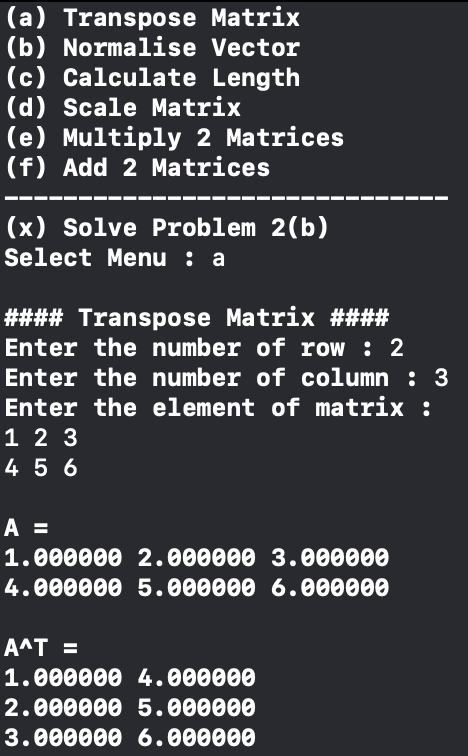
\includegraphics[width=\textwidth]{img/prj0/a.png}
        \caption{Result Image}
        \label{fig:image}
    \end{subfigure}
    \caption{\texttt{transposeMatrix()}}
\end{figure}
\pagebreak

(b) \texttt{normalizeVector(v, n)}: normalise the $n$-dimensional vector $\mathbf{v}$ and return the result\\
Since normalised vector is calculated by dividing all entries by its length, the code below returns the normalised vector $\mathbf{v}$.
\begin{minted}[linenos, fontsize=\small]{c}
double** normalizeVector(double** v, int n) {
    double** w;
    double len = calculateLength(v, n);

    w = allocateMemory(n, 1);
    for (int i = 0; i < n; i++)
        w[i][0] = v[i][0] / len;

    return w;
}
\end{minted}
\begin{figure}[h]
    \centering
    \begin{subfigure}[b]{0.45\textwidth}
        \centering
        \begin {align*}
        \mathbf{v} &= \begin{bmatrix}
            1\\-1
        \end{bmatrix}\\
        ||\mathbf{v}|| &= \sqrt{(1)^2+(-1)^2}\\
        \therefore \hat{\mathbf{v}} &= \begin{bmatrix}
            \frac{1}{\sqrt{2}}\\-\frac{1}{\sqrt{2}}
        \end{bmatrix}\\
        \hat{\mathbf{v}} &\approx \begin{bmatrix}
            0.707107\\-0.707107
        \end{bmatrix}\\
        \end {align*}
        \caption{Equation}
        \label{fig:equation}
    \end{subfigure}
    \hfill
    \begin{subfigure}[b]{0.45\textwidth}
        \centering
        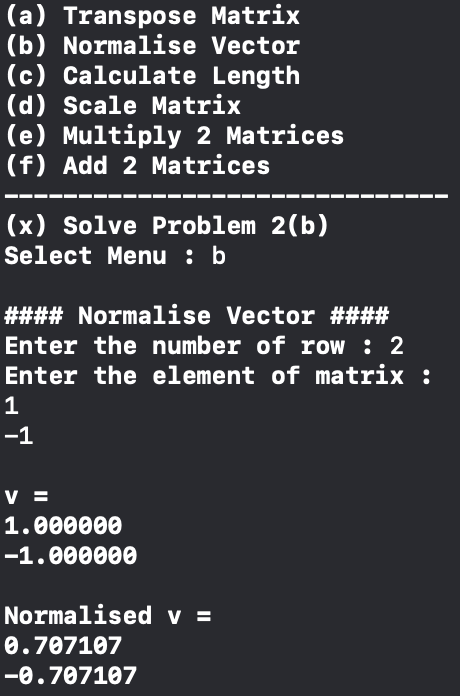
\includegraphics[width=\textwidth]{img/prj0/b.png}
        \caption{Result Image}
        \label{fig:image}
    \end{subfigure}
    \caption{\texttt{normalizeVector()}}
\end{figure}
\pagebreak

(c) \texttt{calculateLength(v, n)}: calculate the length of the $n$-dimensional vector $\mathbf{v}$ and return the result\\
Since length of vector is calculated by square root of the sum of the square of all entries, the code below returns the length of vector $\mathbf{v}$.
\begin{minted}[linenos, fontsize=\small]{c}
double calculateLength(double** v, int n) {
    double len = 0.0;
    
    for (int i = 0; i < n; i++) {
        len += v[i][0] * v[i][0];
    }
    len = sqrt(len);
    
    return len;
}
\end{minted}
\begin{figure}[h]
    \centering
    \begin{subfigure}[b]{0.45\textwidth}
        \centering
        \begin {align*}
        \mathbf{v} &= \begin{bmatrix}
            1\\7\\4
        \end{bmatrix}\\
        ||\mathbf{v}|| &= \sqrt{1^2+7^2+4^2}\\
        ||\mathbf{v}|| &= \sqrt{66}\\
        ||\mathbf{v}|| &\approx 8.124038
        \end {align*}
        \caption{Equation}
        \label{fig:equation}
    \end{subfigure}
    \hfill
    \begin{subfigure}[b]{0.45\textwidth}
        \centering
        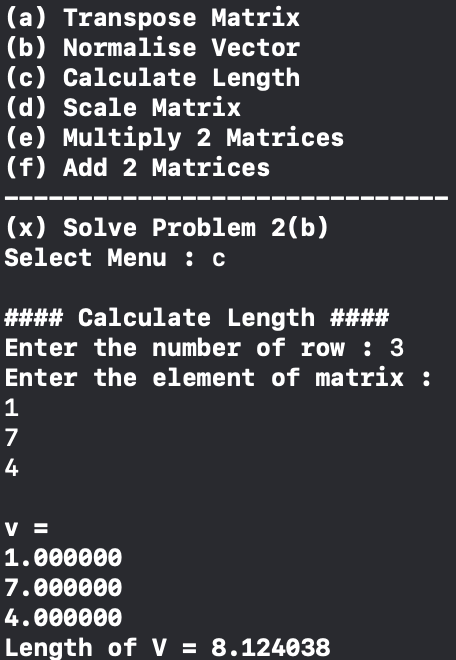
\includegraphics[width=\textwidth]{img/prj0/c.png}
        \caption{Result Image}
        \label{fig:image}
    \end{subfigure}
    \caption{\texttt{calculateLength()}}
\end{figure}
\pagebreak

(d) \texttt{scaleMatrix(A, m, n, c)}: scale the $m \times n$ matrix $A$ with scalar $c$\\
The code below returns the matrix $A$ scaled by $c$ by multiplying all entries in $A$ by $c$.
\begin{minted}[linenos, fontsize=\small]{c}
double** scaleMatrix(double** A, int m, int n, double c) {
    double** cA = allocateMemory(m, n);
    for (int i = 0; i < m; i++) {
        for (int j = 0; j < n; j++) {
            cA[i][j] = c * A[i][j];
        }
    }
    
    return cA;
}
\end{minted}
\begin{figure}[h]
    \centering
    \begin{subfigure}[b]{0.45\textwidth}
        \centering
        \begin {align*}
        3.14\begin{bmatrix}
            1&3&2&4\\3&5&4&5
        \end{bmatrix} = \begin{bmatrix}
                3.14&9.42&6.28&12.56\\
                9.42&15.7&12.56&18.84
            \end{bmatrix}
        \end {align*}
        \caption{Equation}
        \label{fig:equation}
    \end{subfigure}
    \hfill
    \begin{subfigure}[b]{0.45\textwidth}
        \centering
        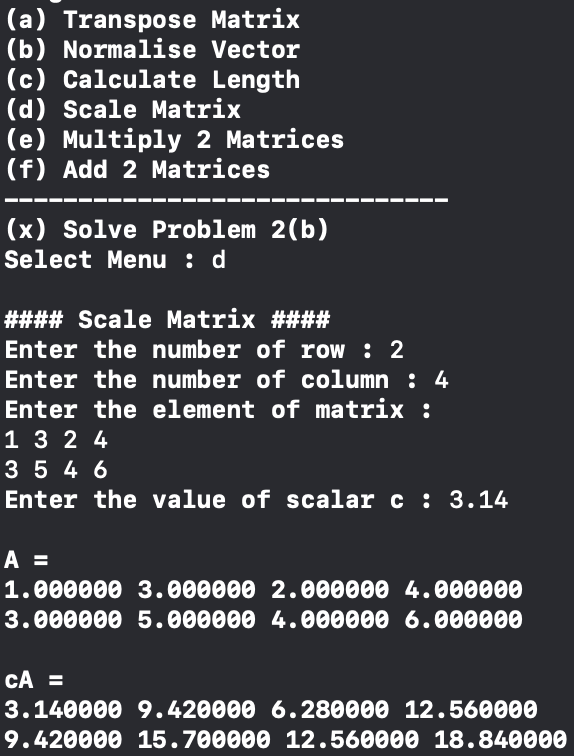
\includegraphics[width=\textwidth]{img/prj0/d.png}
        \caption{Result Image}
        \label{fig:image}
    \end{subfigure}
    \caption{\texttt{scaleMatrix()}}
\end{figure}
\pagebreak

(e) \texttt{multiplyTwoMatrices(A, m, n, B, l, k)}: for $m \times n$ matrix $A$ and $l \times k$ matrix $B$, calculate and return $AB$. Return \texttt{null} if multiplication is impossible.\\
The code below returns the multiplication between matrix $A$ and $B$ or \texttt{NULL} if multiplication is impossible.
\begin{minted}[linenos, fontsize=\small]{c}
double** multiplyTwoMatrices(double** A, int m, int n, double** B, int p, int q) {
    if (n != p) return NULL;
    
    double** AB = allocateMemory(m, n);

    for (int i = 0; i < m; i++) {
        for (int j = 0; j < q; j++) {
            AB[i][j] = 0;
            for (int k = 0; k < p; k++) {
                AB[i][j] += A[i][k] * B[k][j];
            }
        }
    }
    
    return AB;
}
\end{minted}
\begin{figure}[h]
    \centering
    \begin{subfigure}[b]{\textwidth}
        \centering
        \begin {align*}
        \begin{bmatrix}
            1&2&3\\4&5&6
        \end{bmatrix}\begin{bmatrix}
            1&2&3&4&5&6&7\\8&9&10&11&12&13&14\\15&16&17&18&19&20&21
        \end{bmatrix}
        = \begin{bmatrix}
            62&68&74&80&86&92&98\\
            134&149&164&179&194&209&224
        \end{bmatrix}
        \end {align*}
        \caption{Equation}
        \label{fig:equation}
    \end{subfigure}
    \hfill
    \begin{subfigure}[b]{0.45\textwidth}
        \centering
        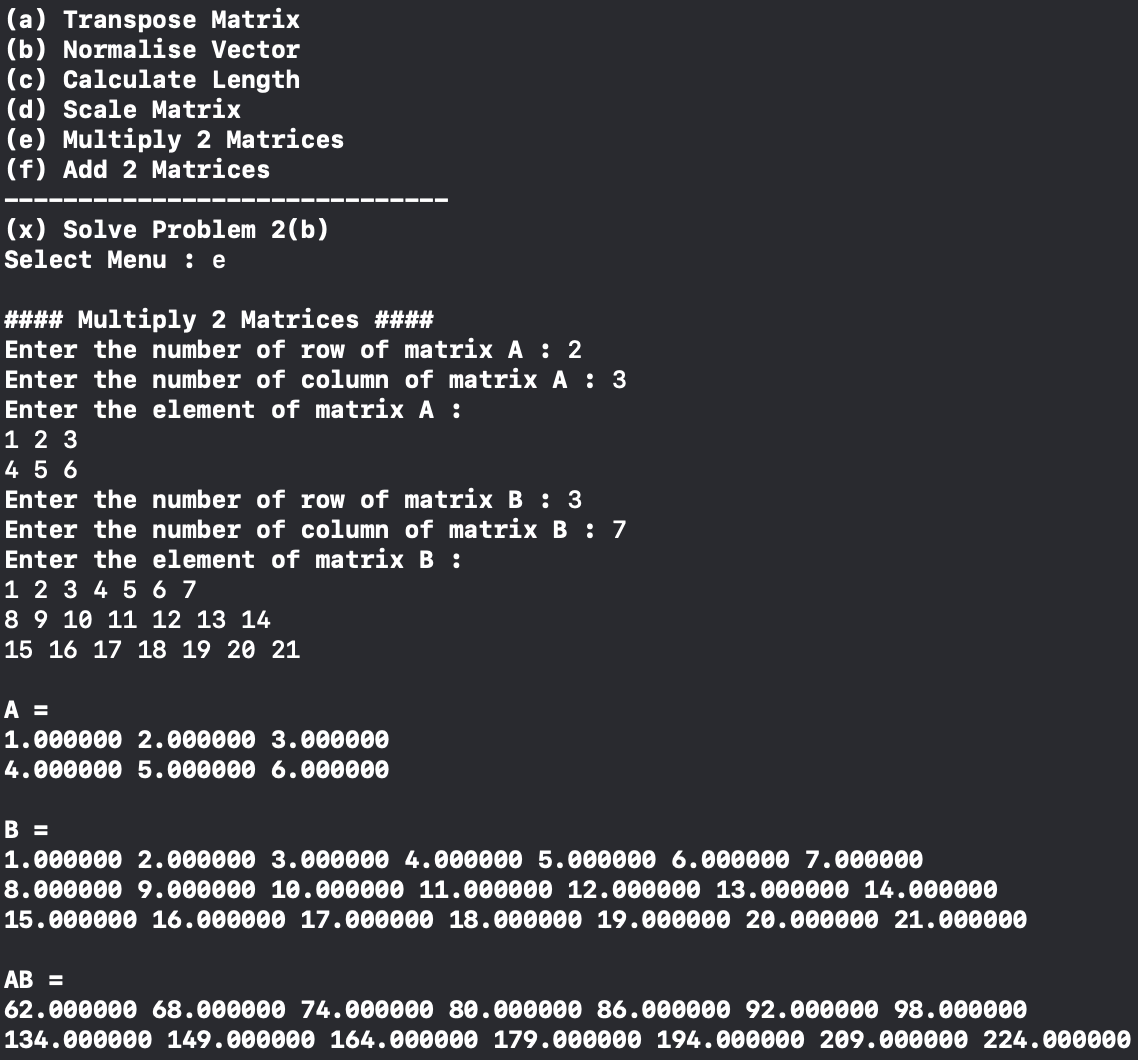
\includegraphics[height=6.7cm]{img/prj0/e.png}
        \caption{Result Image}
        \label{fig:image}
    \end{subfigure}
    \hfill
    \begin{subfigure}[b]{0.45\textwidth}
        \centering
        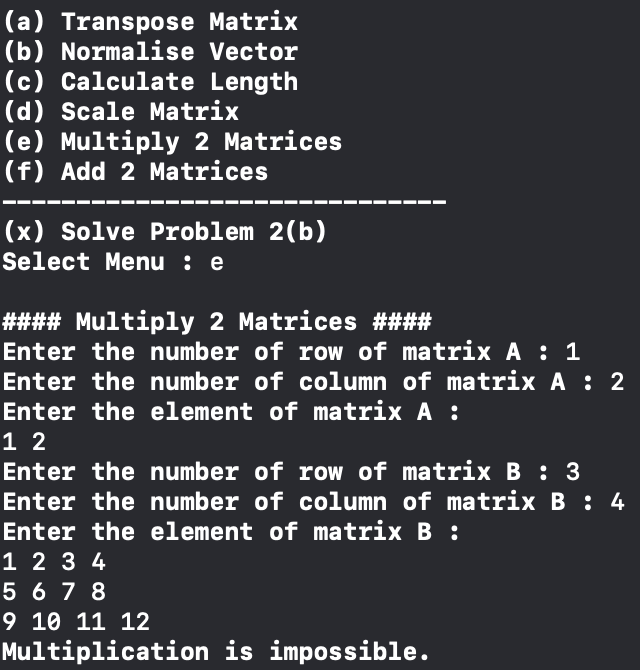
\includegraphics[height=6.7cm]{img/prj0/e-null.png}
        \caption{Result Image When Multiplication is Impossible}
        \label{fig:image}
    \end{subfigure}
    \caption{\texttt{multiplyTwoMatrices()}}
\end{figure}
\pagebreak

(f) \texttt{addTwoMatrices(A, m, n, B, l, k)}: for $m \times n$ matrix $A$ and $l \times k$ matrix $B$, calculate and return $A + B$. Return \texttt{null} if addition is impossible.\\
The code below returns the addition between matrix $A$ and $B$ or \texttt{NULL} if addition is impossible.
\begin{minted}[linenos, fontsize=\small]{c}
double** addTwoMatrices(double** A, int m, int n, double** B, int l, int k) {
    if (m != l || n != k) return NULL;
    
    double** C = allocateMemory(m, n);
    for (int i = 0; i < m; i++) {
        for (int j = 0; j < n; j++) {
            C[i][j] = A[i][j] + B[i][j];
        }
    }
    
    return C;
}
\end{minted}
\begin{figure}[h]
    \centering
    \begin{subfigure}[b]{\textwidth}
        \centering
        \begin {align*}
        \begin{bmatrix}
            1&2&3\\4&5&6
        \end{bmatrix}+\begin{bmatrix}
            7&8&9\\10&11&12
        \end{bmatrix}
        = \begin{bmatrix}
            8&10&12\\14&16&18
        \end{bmatrix}
        \end {align*}
        \caption{Equation}
        \label{fig:equation}
    \end{subfigure}
    \hfill
    \begin{subfigure}[b]{0.45\textwidth}
        \centering
        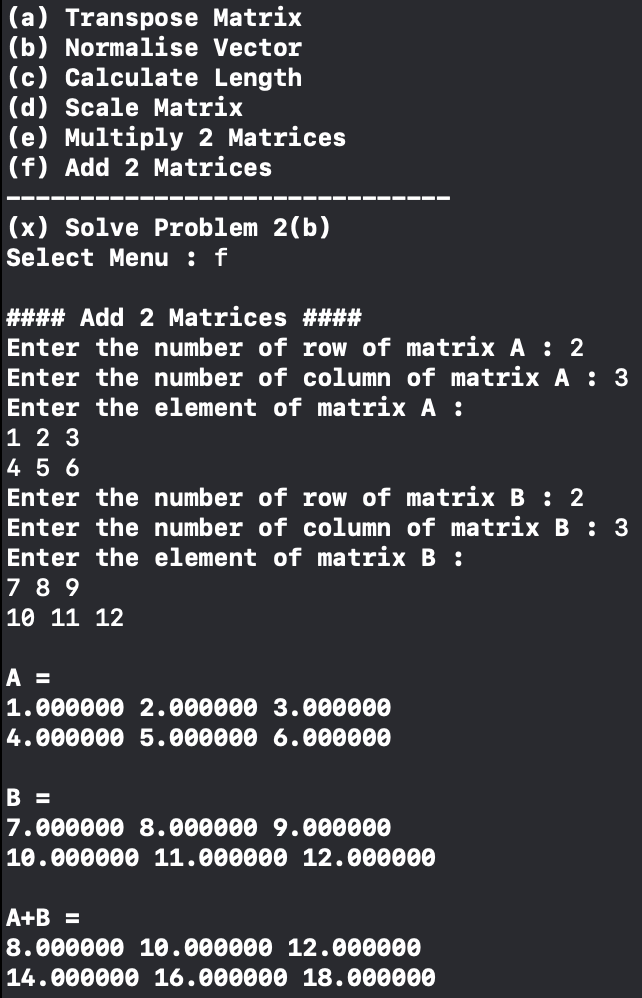
\includegraphics[height=8cm]{img/prj0/f.png}
        \caption{Result Image}
        \label{fig:image}
    \end{subfigure}
    \hfill
    \begin{subfigure}[b]{0.45\textwidth}
        \centering
        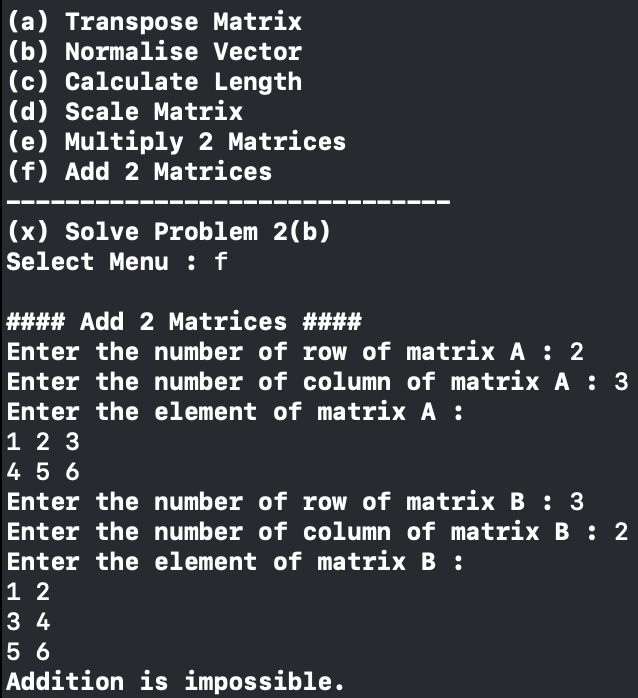
\includegraphics[height=8cm]{img/prj0/f-null.png}
        \caption{Result Image When Addition is Impossible}
        \label{fig:image}
    \end{subfigure}
    \caption{\texttt{addTwoMatrices()}}
\end{figure}
\pagebreak


\subsubsection{2.}
(a) Test the correctness of each of the function you wrote in 1.\\
Already done in above.\\

(b) For given $n\times n$ matrices $A$ and $\tilde{H}$, normalize each column of $\tilde{H}$ (let $H$ be this normalized matrix).
Then, calculate $B = H^T A^H$, and then, $C = HBH^T$.
\begin{minted}[linenos, fontsize=\small]{c}
void problem2b() {
    double a[2][2] = {
        {1, 2},
        {3, 4}
    };
    
    double tildeH[2][2] = {
        {1, 1},
        {1, -1}
    };
    
    double** A = allocateMemory(2, 2);
    for (int i = 0; i < 2; i++)
        for (int j = 0; j < 2; j++)
            A[i][j] = (double) a[i][j];
    printMatrix(A,2,2,"A");
    
    double** TildeH = allocateMemory(2, 2);
    for (int i = 0; i < 2; i++)
        for (int j = 0; j < 2; j++)
            TildeH[i][j] = (double) tildeH[i][j];
    printMatrix(TildeH,2,2,"Tilde H");
    
    double** H = normalizeMatrix(TildeH, 2, 2);
    printMatrix(H, 2, 2, "H");
    
    double** HT = transposeMatrix(H, 2, 2);
    
    double** B = multiplyTwoMatrices(HT, 2, 2, A, 2, 2);
    B = multiplyTwoMatrices(B, 2, 2, H, 2, 2);
    printMatrix(B, 2, 2, "B");
    
    double** C = multiplyTwoMatrices(H, 2, 2, B, 2, 2);
    C = multiplyTwoMatrices(C, 2, 2, HT, 2, 2);
    printMatrix(C, 2, 2, "C");

    releaseMemory(A, 2);
    releaseMemory(TildeH, 2);
    releaseMemory(H, 2);
    releaseMemory(HT, 2);
    releaseMemory(B, 2);
    releaseMemory(C, 2);
}
\end{minted}
\begin{figure}[h]
    \centering
    \begin{subfigure}[b]{0.4\textwidth}
        \centering
        \begin {align*}
        A &= \begin{bmatrix}
            1&2\\3&4
        \end{bmatrix}\\
        \tilde{H} &= \begin{bmatrix}
            1&1\\1&-1
        \end{bmatrix}\\
        H &= \begin{bmatrix}
            \frac{1}{\sqrt{2}}&\frac{1}{\sqrt{2}}\\
            \frac{1}{\sqrt{2}}&-\frac{1}{\sqrt{2}}
        \end{bmatrix}\\\\
        B &= H^TAH\\
        &= \begin{bmatrix}
            \frac{1}{\sqrt{2}}&\frac{1}{\sqrt{2}}\\
            \frac{1}{\sqrt{2}}&-\frac{1}{\sqrt{2}}
        \end{bmatrix}\begin{bmatrix}
            1&2\\3&4
        \end{bmatrix}\begin{bmatrix}
            \frac{1}{\sqrt{2}}&\frac{1}{\sqrt{2}}\\
            \frac{1}{\sqrt{2}}&-\frac{1}{\sqrt{2}}
        \end{bmatrix}\\
        &=\begin{bmatrix}
            5&-1\\-2&0
        \end{bmatrix}\\\\
        C &= HBH^T\\
        &= \begin{bmatrix}
            \frac{1}{\sqrt{2}}&\frac{1}{\sqrt{2}}\\
            \frac{1}{\sqrt{2}}&-\frac{1}{\sqrt{2}}
        \end{bmatrix}\begin{bmatrix}
            5&-1\\-2&0
        \end{bmatrix}\begin{bmatrix}
            \frac{1}{\sqrt{2}}&\frac{1}{\sqrt{2}}\\
            \frac{1}{\sqrt{2}}&-\frac{1}{\sqrt{2}}
        \end{bmatrix}\\
        &=\begin{bmatrix}
            1&2\\3&4
        \end{bmatrix}
        \end {align*}
        \caption{Equation}
        \label{fig:equation}
    \end{subfigure}
    \hfill
    \begin{subfigure}[b]{0.5\textwidth}
        \centering
        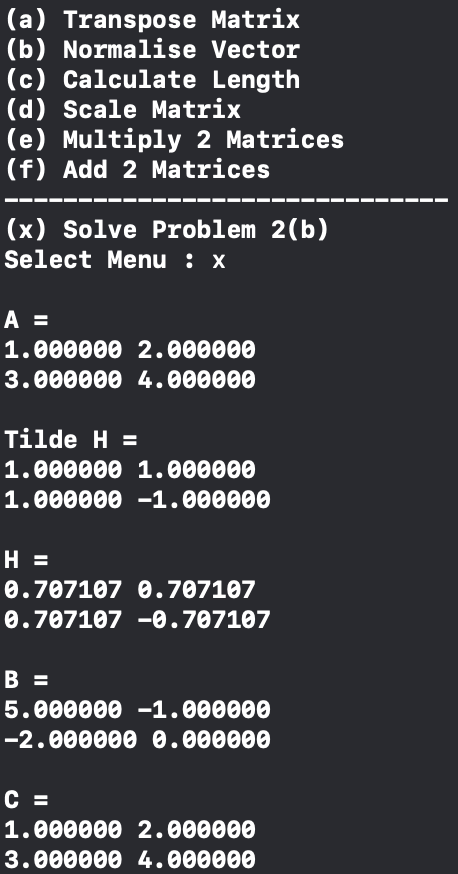
\includegraphics[width=\textwidth]{img/prj0/x.png}
        \caption{Result Image}
        \label{fig:image}
    \end{subfigure}
    \caption{\texttt{problem2b()}}
\end{figure}

\end{document}